% - CRS optimisation in muon channel
Same strategy of CRS is applied to muon channel. Through the optimization cut, higher signal to background 
ratio invariant B mass plot was obtained.

\begin{figure}[]
    \centering
    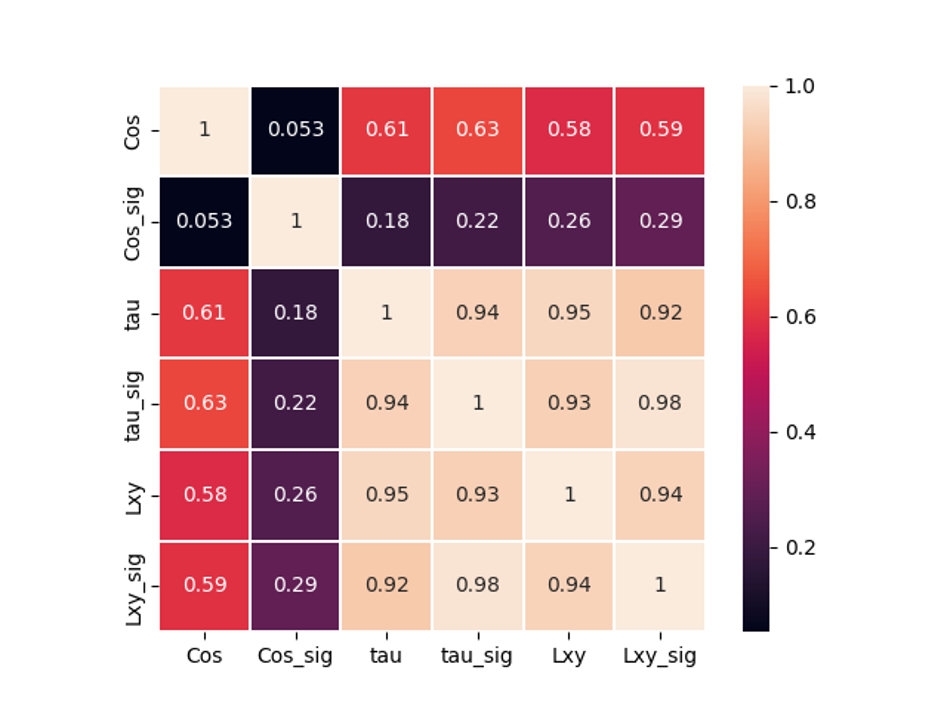
\includegraphics[width=0.45\textwidth]{figures/CRSVarCorrs_muon_Lowq2.png}
    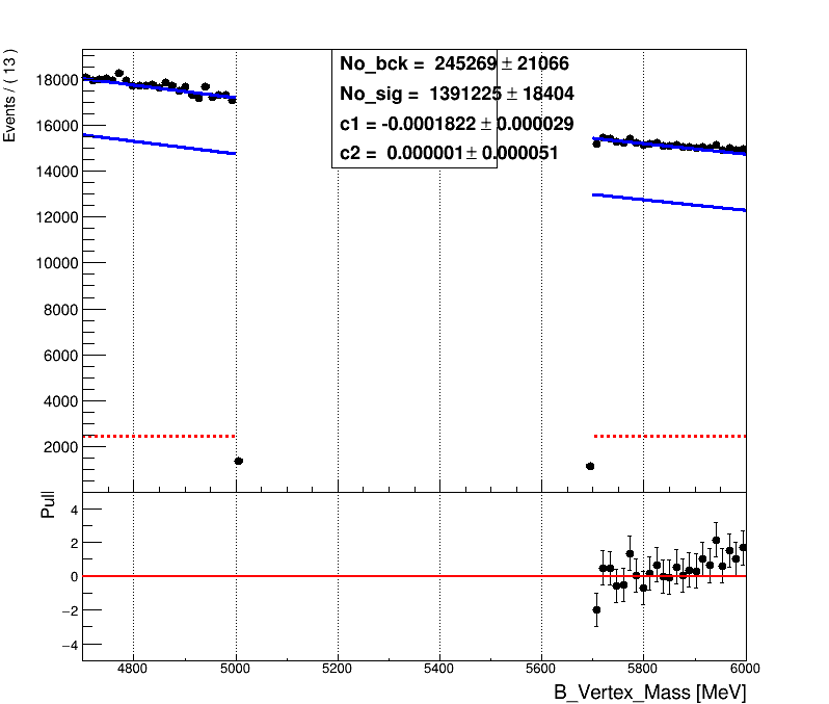
\includegraphics[width=0.35\textwidth]{figures/SidebandFit_CRSoptimisation_muon_Lowq2.png}
    \caption{{\textit{Right plot}}: The linear correlation coefficients between the various
    CRS variables in muon channel.
    {\textit{Left plot}}: A blinded extended-likelihood fit to the invariant mass in the
    low-$q^{2}$ signal region of muon channel. Here the background shape is modelled by an exponential
    (combinatorial component) and a wide Gaussian (misreconstructed B component).
    Below the pulls for the fit are also shown for the high-mass sideband.
    }
    \label{fig:CorrAndSBFit_muon}
\end{figure}

% - Introduction of CRS optimisation in muon channel
We first calculate the number of background events from the sideband fit. The blinded signal region of the 
low-$q^{2}$ data is defined as $m_{B} \in [5.0, 5.7]$\,GeV, whereas the sideband is defined as the region 
$m_{B} \in [4.7, 5.0] \cup [5.7, 6.0]$\,GeV (Fig. \ref{fig:CorrAndSBFit_muon}).

\begin{figure}[]
    \centering
    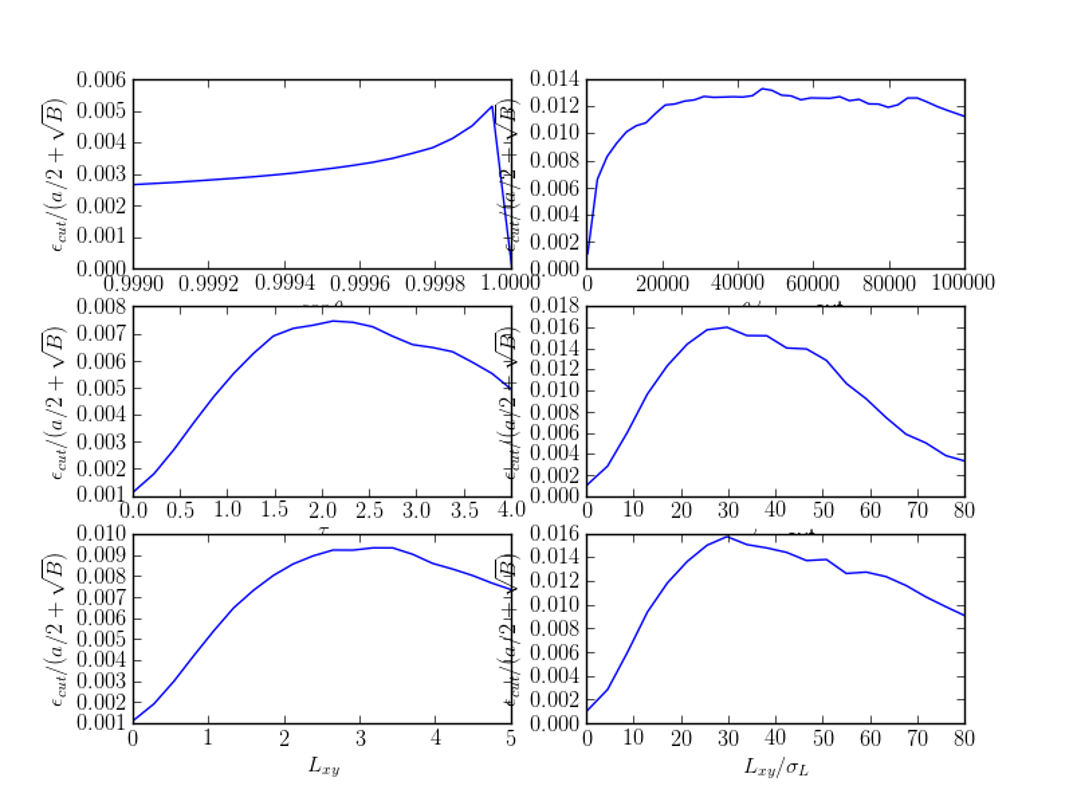
\includegraphics[width = 0.44\textwidth]{figures/PunziScan_muon_Lowq2.png}
    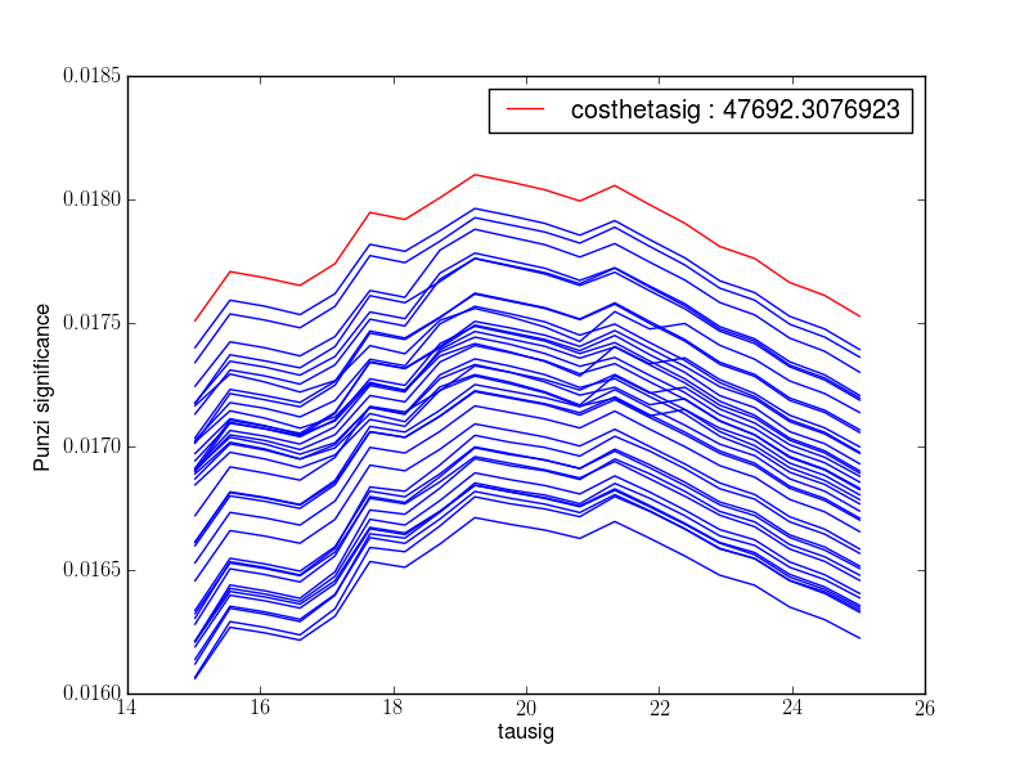
\includegraphics[width = 0.47\textwidth]{figures/2DPunziOpt_muon_Lowq2.png}
    \caption{
    {\textit{Left plot}}: Punzi significance scans for each of the $6$ variables in the CRS optimisation,
    here the $\tau$ significance value has the peak Punzi significance.
    {\textit{Right plot}}: 2D optimisation performed by scanning the Punzi significance of
    $\cos \theta$ significance cuts, for a given cut on the $\tau$ significance.}
    \label{fig:PunziScans_muon}
\end{figure}

To obtain the maximum sensitivity, 1D punzi significance scans in the low-$q^{2}$ region was performed (Fig. \ref{fig:PunziScans_muon}). 
Maximum punzi significance was observed at $\tau/\sigma_{\tau} > 29.47$. Having chosen the $\tau$ significance as the 
first variable in the 2D CRS optimization, the second variable is chosen as least correlated variable with $\tau$ significance
using correlation matrix (Fig. \ref{fig:CorrAndSBFit_muon}). 2D optimization was then performed and maximum thresholds were found to be $\tau/\sigma_{\tau} >  19.21, 
\cos \theta/\sigma_{\cos \theta} > 47692.31$ (Fig. \ref{fig:PunziScans_muon}).

\begin{figure}
    \centering
    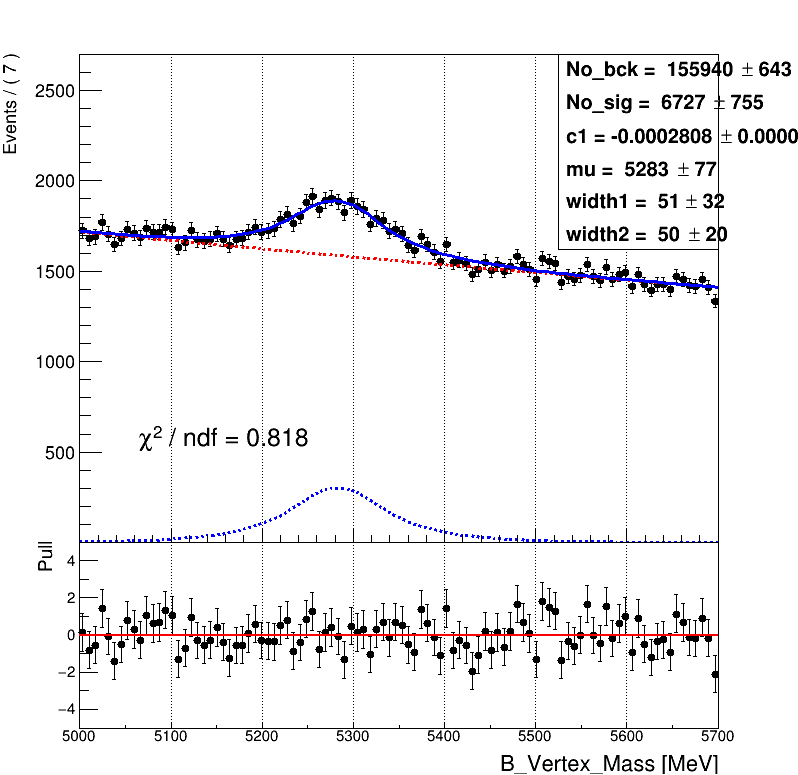
\includegraphics[width = 0.4\textwidth]{figures/B_masses_cutflow_JPsi_highq2_datafit_muon.png}
    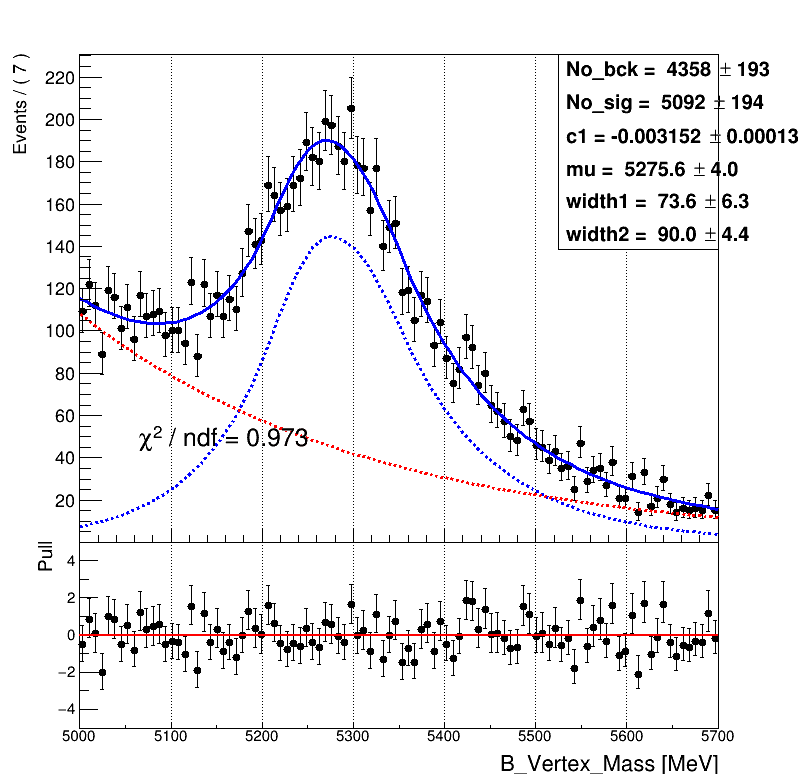
\includegraphics[width = 0.4\textwidth]{figures/BmassFit_Jpsi_Data_Highq2_CRS_muon.png}
    \caption{(Left) Extended likelihood fits to the invariant B mass, with only the preselection applied,
    here signal is shown in blue and background in red. The fit results are also shown.
    (Right) Extended likelihood fits to the invariant B mass, with the preselection and
    additional CRS applied, here signal is shown in blue and background in red.
    The fit results are also shown. }
    \label{fig:CRSvsCutflowFits_muon}
\end{figure}

The optimized CRS cuts was then applied to the high-$q^{2}$ data to demonstrate the discriminating power.
For the high-$q^{2}$, we observe a clearer emergence of the $B$ mass peak from the overwhelming
background. Extended likelihood fits to the invariant mass of $B$ candidates, with and without the CRS applied, are shown for comparison (Fig. \ref{fig:CRSvsCutflowFits_muon}).
Similar to electron channel, the CRS gives us a much better handle on the functional form of the signal shape and 
allows us to better understand the contribution of the misreconstructed B background.